\documentclass{article}
\usepackage[utf8]{inputenc}
\usepackage{listings}
\usepackage{color}
\usepackage[framed]{mcode}
\usepackage{graphicx}
\usepackage{amsmath}
\graphicspath{ {images/} }
\usepackage{floatrow} %figure captions at bottom
\usepackage{mathtools}
\DeclarePairedDelimiter\ceil{\lceil}{\rceil}
\DeclarePairedDelimiter\floor{\lfloor}{\rfloor}

\title{Technical information about the inner workings of MountainSort}
\author{Jeremy Magland and Alex Barnett}
\date{February 2016}

\begin{document}

\maketitle

\section{Notation and conventions}

\begin{itemize}
    \item[] $M$ - number of channels
    \item[] $N$ - number of timepoints
    \item[] $K$ - number of neurons/clusters
    \item[] $T$ - extracted clip size (timepoints)
    \item[] $L$ - number of events
\end{itemize}

We use $1$-based indexing for timepoints and neuron numbering. The center of an event clip of length $T$ timepoints in $\floor*{\frac{T+1}{2}}$.

\section{Sorting pipeline for small arrays}

\begin{figure}[h]
\caption{Sorting pipeline for small and large electrode arrays}
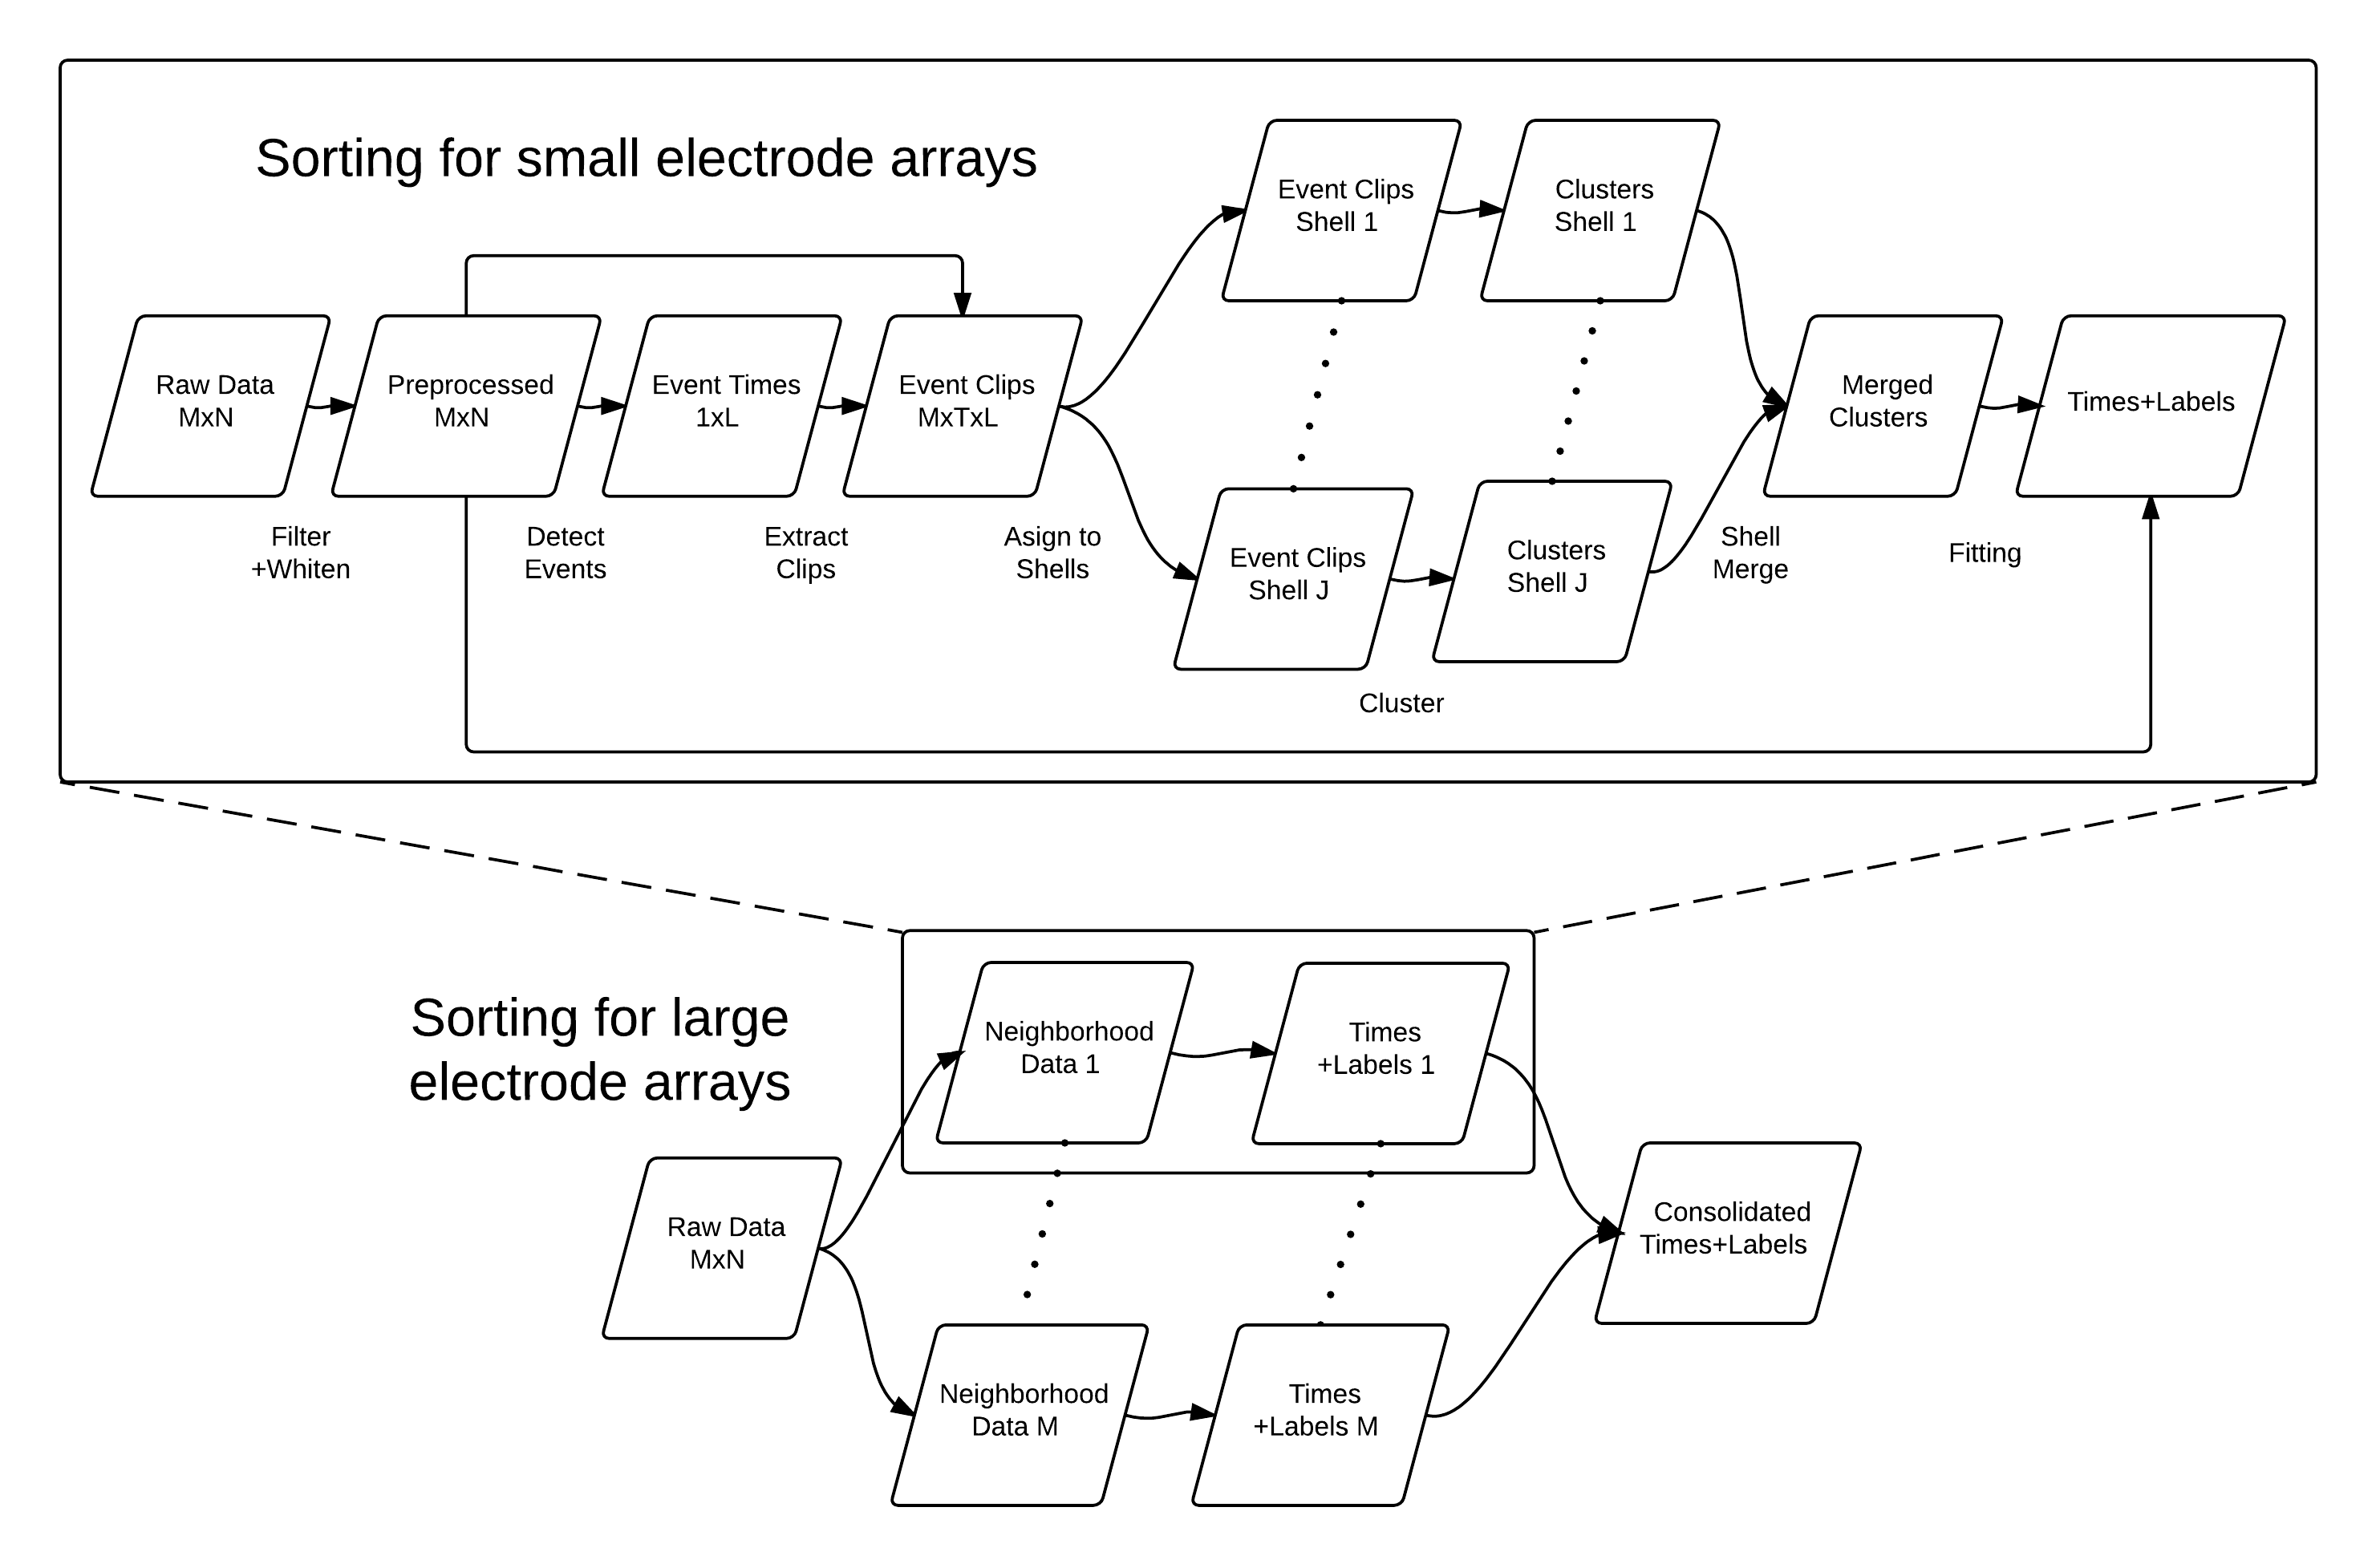
\includegraphics[width=4.5in]{pipelines.png}
\end{figure}

\subsection{Bandpass filter}

\subsection{Whitening}

The goal of whitening is to remove correlations between channels and normalize each channel to have unit variance. Let $X_{m,n}$ be the bandpass filtered, non-whitened signal for channel $m$ at the $n$th timepoint ($m=1,\dots,M$ and $n=1,\dots,N$). The covariance matrix is
$$C=X X',$$
which we would like to be the identity matrix. Let
$X=USV'$ be the singular value decomposition where $U$ is $M\times M$, $V$ is $N\times M$ and $S$ is the diagonal matrix of $M$ singular values.
Then the transformed (whitened) data is defined to be
$$\tilde{X}=US^{-1}U'X.$$
This is equal to $UV'$ which has identity covariance matrix.

Note that $\tilde{X}$ could be replaced by $W\tilde{X}$ for any unitary transformation $W$. However, the above choice is preferred in the sense that it largely preserves the channel locality (not sure how to make this claim precise) which is important when detecting super-threshold spikes.

Whitening effectively suppresses signal across channels that recurs throughout the data set. For example, if there is a common mode across many or all of the channels, this is suppressed or almost completely removed. Although actual spike events repeat throughout, the assumption is that each individual spike type contributes very little to the overall variance of the data, and therefore should not be significantly suppressed as a part of whitening.

Here is a brief MATLAB code that verifies the above formulae.

\begin{lstlisting}
A=rand(4,1000); % 4 channels, 1000 timepoints
[U,S,V]=svd(A,'econ'); % singular value decomposition
A_tilde=U*inv(S)*U'*A; % whitening operation, equivalent to U*V'
disp(A_tilde*A_tilde'); % should be identity matrix
disp(A_tilde-U*V'); % Should be zero
\end{lstlisting}

After whitening, since each channel will have unit variance, the detection threshold may be set in units of standard deviations from the mean.

\subsection{Detection}

The purpose of detection is to identify timepoints where spiking events may have occurred. The output is an array of timepoints ideally located at the peak amplitudes of the spikes. Here we focus on the case where we are detecting only positive amplitude spikes on a single channel, but the method can easily be adapted to handle spikes in the absolute value of the signal across one or more channels.

An event is flagged whenever the signal exceeds $\mu_{\text{detect}}$, a threshold parameter in units of standard deviations above the mean. A typical choice is $\mu_{\text{detect}}=4$. However, a spike will usually involve several suprathreshold timepoints, and we only want to flag one event per spike. Therefore we also need a parameter $\tau_{\text{detect}}$ specifying a minimum number of timepoints separating two events. We say an event occurs at timepoint $t$ if the signal $S(t)$ exceeds
$\mu_{\text{detect}}$ and $S(t)\geq S(t')$ whenever $\|t-t'\|\leq \tau_{\text{detect}}$. We assume there are no "ties", since equality to machine precision is extremely unlikely. However this does not pose a problem for our particular code implementation as the latter instance will always be used.

Here is a MATLAB code that implements this simple algorithm together with the output plot. Note that due to the \emph{for loop} this is better written in C.

\begin{lstlisting}
function test_sample_detect
N=800;
detect_interval=15;
detect_threshold=4;
X=randn(1,N)+create_triangular_spikes(N,10,5,30);
times=sample_detect(X,detect_threshold,detect_interval);
figure; plot(1:N,X,'k'); hold on;
for j=1:length(times)
    plot([times(j),times(j)],ylim,'r--');
end;
plot(xlim,[detect_threshold,detect_threshold],'b--');
end

function times=sample_detect(X,detect_threshold,detect_interval)
N=length(X);
use_it=zeros(1,N);
best_ind=1;
best_val=X(1);
candidates=find(X>=detect_threshold);
for tt=candidates
    if (best_ind<tt-detect_interval)
        [~,best_ind]=max(X(tt-detect_interval:tt-1));
        best_ind=best_ind+tt-detect_interval-1;
        best_val=X(best_ind);
    end;
    if (X(tt)>=best_val)
        use_it(tt)=1;
        use_it(best_ind)=0;
        best_ind=tt;
        best_val=X(tt);
    end;
end;

times=find(use_it==1);
end

function X=create_triangular_spikes(N,num,amp,len)
X=zeros(1,N);
spike_shape=amp*(1-abs(linspace(-1,1,len)));
for n=1:num
    loc=randi([1,N-len+1]);
    X(loc:loc+len-1)=spike_shape;
end;
end
\end{lstlisting}

\begin{figure}[h]
\caption{MATLAB output of test\_sample\_detect.m}
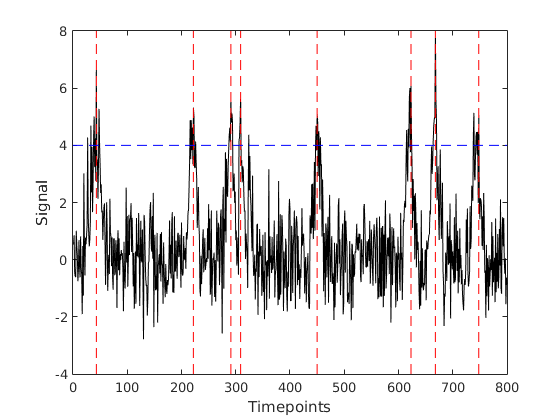
\includegraphics[width=3in]{test_sample_detect.png}
\end{figure}

\subsection{Feature extraction}

Prior to sorting of events, dimension reduction via principal component (PCA) feature extraction is performed. There are two primary advantages. The first is simply computational as the subsequent steps are substantially more efficient when operating in, for example, $12$ dimensions rather than $M\times T$ dimensions where $M$ is the number of channels and $T$ is the number of time steps in an extracted event clip (centered at the detection timepoint). The second advantage is reduction of noise and artifacts, and to some degree the problem of multiple events occurring within the time window. This is because the principal components primarily capture the features that are common to large numbers of events.

Let $C$ be the $MT \times L$ array of extracted event clips, where $MT$ is the vectorized length of a single clips, and $L$ is the number of detected events. Principal components are extracted using eigenvalue decomposition. If $D$ is the diagonal matrix of $MT$ eigenvalues of $XX'$ in descending order and $U$ is the $M\times M$ matrix of corresponding eigenvectors in columns, then the $M\times N$ matrix of PCA features is given by $\tilde{F}=U'D$. The first $n_{\text{features}}$ rows of $M$, denoted by $F$, is the $n_{\text{features}}\times N$ array of features which is the input to the subsequent clustering steps.

\subsection{Clustering in shells}

Event clustering is a central step in spike sorting. The goal is to provide integer labels to events such that ideally (a) spikes from the same neuron are labeled the same and (b) spikes with the same label arise from the same neuron. The former criterion corresponds to proper splitting of clusters, and the latter to proper merging. In addition to false splitting and false merging, there are three kinds of errors that relate to the separation of signal and noise. First, clusters of pure noise may be present. Second, pure noise or outlier events may be included in a cluster which otherwise corresponds to a unique neuron. Finally, events may be misclassified based on corruption by noise or artifact.

The choice of detection threshold is crucial for separating signal from noise. If the threshold is set too high, low amplitude clusters and/or events will be missed. On the other hand, if the threshold is too low then noise clusters will be detected, and more problematically, low amplitude clusters will be merged into the noise cluster. If two valid clusters are both merged into the same noise cluster then they may also be incorrectly merged with one another.

To address these issues we propose a method to cluster in a series of amplitude shells followed by a cluster merging procedure. For now we handle the cause of strictly positive amplitude peaks, but the scheme may be adapted to the case where both positive and negative amplitude events are detected. Let $0=\mu_{1-}<\mu_{2-}<\dots<\mu_{n-}$ and $\mu_{1+}<\mu_{2+}<\dots<\mu_{n+}=\infty$ be a series of lower and upper amplitude bounds, respectively, with $\mu_{j-}<\mu_{j+}$. Let
$$S_j=\{e_l:\mu_{j-}\leq a(e_l)<\mu_{j+}\}$$
be the set of events in the $j$th shell, where $a(e_l)$ is the peak amplitude of the $l$th event. It is important that these shells are not mutually exclusive ($\mu_{j+}>\mu_{j+1-}$) so that merging in the subsequent step is possible.

Clustering is then applied to each shell independently. We use the ISO-SPLIT algorithm [ref] which does not depend on any adjustable parameters, such as the \emph{a priori} number of clusters or a length scale. This is a density-based and model-free algorithm that assumes that each cluster is unimodal in the sense that it has a single region of peak density and that any two clusters are separated by a hyperplane of relatively lower density.

\subsection{Shell merging}

Clusters in adjacent shells are merged as follows. Let $S_j$ denote the set of events in the $j$th shell and let $C_{j,k}\subset S_j$ denote the $k$th cluster in the $j$th shell. Then we define the agreement between clusters $C_{j,k}$ and $C_{j+1,k'}$ to be
$$\eta_{j,k,j+1,k'}=\frac{\#\{A\cap B\}}{\#\{A\cup B\}}$$ where
$A=C_{j,k}\cap S_{j+1}$ and $B=C_{j+1,k'}\cap S_j$. In words, it is the fractional agreement in the overlap region of the two shells. These two clusters are then merged if 
$$\eta_{j,k,j+1,k'}>\tau_{\text{merge}}$$  threshold $\tau_{\text{merge}}\geq \frac{1}{2}$.

The merged result comprises clusters of the form
$$C_{j,k_1}\cup C_{j+1,k_2}\cup\dots C_{j+a-1,k_a}$$
where the adjacent clusters have been merged. This is well defined due to the following fact: If $C_{j,k}$ can be merged to at most one cluster in shell $j+1$. Indeed, suppose that it is merged to both $C_{j+1,k'}$ and $C_{j+1,k''}$. Then we have
$$\frac{\#\{A\cap B'\}}{\#A}\geq\frac{\#\{A\cap B'\}}{\#\{A\cup B''\}}>\tau_{\text{merge}}\geq\frac{1}{2}$$
and
$$\frac{\#\{A\cap B''\}}{\#A}\geq\frac{\#\{A\cap B''\}}{\#\{A\cup B''\}}>\tau_{\text{merge}}\geq\frac{1}{2}$$
where $A$, $B'$, and $B''$ are defined similar to as above. This implies that $B'=B''$, or equivalently $k'=k''$.

\section{Sorting pipeline for large arrays}

\subsection{Local neighborhoods}

\subsection{Preprocessing and detection}

\subsection{Clustering in local neighborhoods}

\subsection{Cluster consolidation}

The same neuron will typically be identified on more than one channel, and therefore redundancies need to be eliminated. In most cases, each neuron will have a primary electrode on which it loads with greater energy than on any other electrode. Therefore, if cluster $k$ was identified from channel $m_k$ and 
$$\|W_k(m_k,\cdot)\|_2<\mu_{\text{con}} \|W_k(m^\prime,\cdot)\|_2$$
where $W_k$ is the representative cluster
and $m^\prime$ represents some other channel, then we assume that $k$ is a redundant cluster and can therefore be eliminated. Here, $\mu_{\text{con}}<1$ is a tolerance constant (e.g., $\mu_{\text{con}}=0.9$). In other words, we eliminate all clusters whose primary load channel is not the channel used to identify the cluster.

The above heuristic handles most redundancies without the need to compare waveform shapes or firing time agreements. This is important since detection of the same neuron will certainly be of different quality on different channels. However, sometimes a neuron fires with around the same energy on two nearby electrodes. We therefore use a second criterion (in a second pass) to handle these situations. Let $n_{k_1}$ be the number of events classified as type $k_1$ and let $n_{k_1,k_2}$ be the number of these events which are near (within $10$ time points) of an event classified as $k_2$. Let $0<p_{con}\leq 1$ be a \emph{coincidence} threshold (e.g., $p_{con}=0.5$). If $n_{k_1,k_2}>\tau_{con} n_{k_1}$ or $n_{k_1,k_2}>\tau_{con} n_{k_2}$, then we consider $k_1$ and $k_2$ to represent the same neuron and therefore we eliminate either $k_1$ or $k_2$, whichever occurs with less frequency.

Note that \emph{consolidation} is different from \emph{merging}. Merging denotes taking a union of two sets of events, whereas our consolidation simply involves deleting a cluster. This makes sense because we are handling the situation where two clusters (occurring on different channels) actually represent the same neuron, and one can therefore be deleted.

\end{document}
